\documentclass[11pt]{article}
\usepackage[margin=1in]{geometry}
\usepackage{amsmath,amssymb,amsthm}
\usepackage{graphicx}
\usepackage{booktabs}
\usepackage{float}
\usepackage{caption}
\usepackage[hidelinks]{hyperref}
\usepackage[margin=10pt,font=footnotesize,labelfont=bf]{caption}

\DeclareMathOperator{\sech}{sech}
\newcommand{\dd}{\mathrm{d}}
\newcommand{\sgn}{\operatorname{sgn}}

\title{\bfseries Sigmoid--G Alternating Activation (SGAA):\\
A Reciprocal-Derivative Pairing that Limits Gradient Vanishing and Explosion}
\author{SGAA Research Project}
\date{\today}

\begin{document}
\maketitle

\begin{abstract}
\noindent
The logistic sigmoid $\sigma(x)=1/(1+e^{-x})$ has a bounded derivative
$\sigma'(x)=\sigma(x)(1-\sigma(x))\le1/4$. When a deep network uses $\sigma$
as every activation, backpropagated gradients multiply many small factors
$\sigma'(z_\ell)$ and collapse exponentially with depth. We study a simple
alternative: define the antiderivative of the \emph{reciprocal} derivative,
\begin{equation}
  G(x)=\int \frac{1}{\sigma'(x)}\,\dd x = e^{x}-e^{-x}+2x = 2\sinh(x)+2x,
  \qquad
  G'(x)=\frac{1}{\sigma'(x)},
\end{equation}
and use $\sigma$ and $G$ as \emph{alternating} activations. Because
$G'=1/\sigma'$, the product of the two derivatives entering the backprop chain
for an adjacent $(\sigma,G)$ pair is
\begin{equation}
  \sigma'(z_i)\,G'(z_{i+1})=\frac{\sigma'(z_i)}{\sigma'(z_{i+1})},
\end{equation}
which equals $1$ whenever the two pre-activations are similar. On the MNIST
benchmark we compare all-$\sigma$, alternating $\sigma/G$ (both orderings),
ReLU and tanh. Alternating $\sigma/G$ keeps the adjacent-derivative product
$\mathcal{O}(10)$ times closer to $1$ than all-$\sigma$, yields the highest
test accuracy of the saturating schemes, and shows substantially flatter
per-layer gradient norms. The unbounded forward growth of $G$ nevertheless
imposes an activation-explosion limit at large depth that no derivative
rescaling can remove; we characterise this trade-off quantitatively.
\end{abstract}

\section{Introduction}
\label{sec:intro}
Vanishing and exploding gradients are a central obstruction to training deep
networks. For a composition of activations $\phi_\ell$ with derivatives
$\phi'_\ell(z_\ell)$, the error signal is propagated by products of Jacobians;
when every $\phi_\ell=\sigma$ the scalar factors $\sigma'(z_\ell)$ lie in
$(0,1/4]$, and their product vanishes geometrically with depth. Many remedies
exist---careful initialisation, batch normalisation, residual connections,
skew-symmetric weight matrices---but all add parameters or machinery.

We pursue a complementary, algebraic idea that requires no additional
parameters, no dedicated initialisation scheme and no architectural change.
The logistic sigmoid is the common activation whose derivative is expressible
through $\sigma$ itself, $\sigma'(x)=\sigma(x)(1-\sigma(x))$, and hence admits a
closed-form antiderivative for the \emph{reciprocal} derivative.  We define
$G$ by $G'(x)=1/\sigma'(x)$ (Section~\ref{sec:G}) and interleave $\sigma$ and
$G$ as hidden activations.  Consecutive layers contribute
$\sigma'(z_i)G'(z_{i+1})$, a ratio of two numbers in $(0,1/4]$ and therefore
$\mathcal{O}(1)$, rather than the product
$\sigma'(z_i)\sigma'(z_{i+1})\le1/16$ that all-$\sigma$ propagates.  When the
two pre-activations are similar the ratio is exactly $1$, so an alternating
pair can neither vanish nor explode at that layer.

The purpose of this paper is to test whether this algebraic balancing survives
contact with real optimisation.  We derive and verify the closed form of $G$,
give a numerically stable implementation of both $G$ and $G'=1/\sigma'$, and
compare all-$\sigma$, alternating $\sigma/G$ (in both orderings), ReLU and tanh
on MNIST, measuring training curves, per-layer gradient norms and the
derivative-product identity.  We find that $\sigma/G$ alternation keeps the
gradient ratio at $\approx1$ from initialisation, outperforms all-$\sigma$, and
extends the depth to which a sigmoid-based network can be trained---but that
the exponential forward growth of $G$ imposes its own ceiling.

\section{Mathematical background}
\label{sec:theory}

\subsection{The sigmoid and its derivative}
\label{sec:sigmoid}
The logistic sigmoid is
\begin{equation}
  \sigma(x)=\frac{1}{1+e^{-x}},\qquad
  \sigma'(x)=\sigma(x)\bigl(1-\sigma(x)\bigr).
\end{equation}
A useful symmetric form follows from $\sigma(-x)=1-\sigma(x)$:
\begin{equation}
  \sigma'(x)=\sigma(x)\,\sigma(-x),
\end{equation}
which is \emph{exactly} equal to $\sigma(x)(1-\sigma(x))$. This form is the
numerically stable way to evaluate the derivative: for large $|x|$, $\sigma(x)$
rounds to $1$ (or $0$) in single precision and $1-\sigma(x)$ suffers
catastrophic cancellation, whereas $\sigma(x)\sigma(-x)$ computes two bounded
values in $(0,1)$ with no subtraction. Since $\sigma'(x)\in(0,1/4]$, its
reciprocal is in $[4,\infty)$.

\subsection{The reciprocal-derivative antiderivative $G$}
\label{sec:G}
We seek $G$ with $G'(x)=1/\sigma'(x)$. Expanding,
\begin{equation}
  \frac{1}{\sigma'(x)}=\frac{(1+e^{-x})(1+e^{x})}{1}
   = 2+2\cosh x = e^{x}+2+e^{-x}.
\end{equation}
Integrating term by term and choosing $G(0)=0$,
\begin{equation}
  G(x)=\int \frac{\dd x}{\sigma'(x)} = e^{x}-e^{-x}+2x
       = 2\sinh(x)+2x,
  \qquad
  G'(x)=e^{x}+e^{-x}+2=2+2\cosh x=\frac{1}{\sigma'(x)}.
\end{equation}
$G$ is an odd, strictly increasing function with $G(0)=0$, $G'(0)=4$, and
$G$ grows like $\operatorname{sgn}(x)\,e^{|x|}$ for large $|x|$.

\paragraph{Numerically stable evaluation of $G$.}
The formula $2\sinh x+2x$ is accurate for $|x|\lesssim20$; for larger $|x|$ one
exponential dominates and we keep only it, reproducing $G$ to better than
$10^{-8}$ relative accuracy:
\begin{equation}
  G(x)\approx
  \begin{cases}
    2\sinh x+2x, & |x|\le20,\\
    \operatorname{sgn}(x)\,e^{|x|}+2x, & |x|>20.
  \end{cases}
\end{equation}
Crucially $G'$ is evaluated as $1/[\sigma(x)\sigma(-x)]$, which never overflows
in the intermediates and remains finite and accurate for $|x|$ up to $\sim88$.
This stability is what makes the alternating scheme trainable in practice.

\subsection{The SGAA derivative-product identity}
\label{sec:identity}
Consider two adjacent hidden layers with pre-activations $z_i$ and $z_{i+1}$,
one using $\sigma$ and the other $G$. Backpropagation multiplies their
derivatives, so the combined factor is
\begin{equation}
  \boxed{\;\sigma'(z_i)\,G'(z_{i+1})=\frac{\sigma'(z_i)}{\sigma'(z_{i+1})}.\;}
\end{equation}
If $z_i=z_{i+1}$ the product is exactly $1$---neither vanishing nor
exploding. More generally, writing $\Delta z=z_i-z_{i+1}$ and using
$(\log\sigma')'=\sigma''/\sigma'=1-2\sigma$,
\begin{equation}
  \sigma'(z_i)G'(z_{i+1})\approx
  \exp\!\bigl[\bigl(1-2\sigma(z_{i+1})\bigr)\Delta z\bigr],
\end{equation}
so the product is $1$ to first order whenever $\Delta z$ is small, and deviates
exponentially only when the pre-activations genuinely differ. The magnitude of
the deviation is governed by the same saturating factor $1-2\sigma(z)$ that
defines the sigmoid's flat tails. This is precisely the quantity the all-$\sigma$
case fails to control: there the product is $\sigma'(z_i)\sigma'(z_{i+1})$, which is
always $\ll1$ once both layers saturate.

\section{Methods}
\label{sec:methods}

\subsection{Network and activation schemes}
We use an MLP with $784$ inputs, $10$ outputs and $L$ hidden layers of width
$W$, written as $\mathrm{Linear}+\phi_\ell$ for $\ell=1,\dots,L$, followed by a
logit layer. All linear layers are Xavier-uniform, bias-zero initialised, so the
\emph{only} variable across runs is the activation scheme:
\begin{center}
\begin{tabular}{ll}
\toprule
scheme & hidden activations $\phi_1,\dots,\phi_L$\\
\midrule
all-$\sigma$        & $\sigma,\sigma,\dots,\sigma$\\
$\sigma/G$ alt      & $\sigma,G,\sigma,G,\dots$\\
$G/\sigma$ alt      & $G,\sigma,G,\sigma,\dots$\\
ReLU                & $\mathrm{ReLU},\mathrm{ReLU},\dots$\\
tanh                & $\tanh,\tanh,\dots$\\
\bottomrule
\end{tabular}
\end{center}

\subsection{Data and training}
MNIST (60k train / 10k test), pixels normalised to $[-1,1]$, read from
\texttt{/root/data/MNIST/raw}.  Adam with learning rate $10^{-3}$, batch size $256$,
cross-entropy loss, no weight decay.  Main comparison: $W=256$, $L=4$, 10
epochs, 3 seeds; we report mean$\pm$std.  Depth sweep: $W=128$, $L\in\{2,4,6,10,16,24,32\}$,
one seed, up to 6 epochs, to probe the gradient/activation behaviour at depth.

\subsection{Diagnostics}
For a fixed diagnostic batch we record, after a forward/backward pass:
\begin{itemize}
  \item per-layer pre-activation gradient norms $\|\partial L/\partial z_\ell\|$
        and the ratio $\|\partial L/\partial z_L\|/\|\partial L/\partial z_1\|$
        (large = exploding, $\ll1$ = vanishing);
  \item the activation magnitude $\max_\ell \|a_\ell\|_\infty$ and whether any
        activation is NaN/Inf (forward explosion detector);
  \item the adjacent derivative products
        $\sigma'(z_i)\cdot\text{deriv}_{\ell+1}(z_{i+1})$ and their deviation
        from $1$;
  \item the adjacent $\sigma'$-similarity
        $\bigl\langle\bigl|\sigma'(z_i)-\sigma'(z_{i+1})\bigr|/\bar\sigma'\bigr\rangle$,
        a direct measure of the hypothesis's precondition.
\end{itemize}

\section{Results}
\label{sec:results}

\subsection{Training comparison}
\label{sec:results-training}
Table~\ref{tab:main} and Figures~\ref{fig:train}--\ref{fig:accbar} summarise the
main comparison ($W=256$, $L=4$, 10 epochs, 3 seeds).  The alternating
$\sigma/G$ scheme is the best of the two sigmoid-based schemes: it reaches a best
test accuracy of $0.9741\pm0.0015$, beating all-$\sigma$
($0.9721\pm0.0014$) and matching the non-saturating baselines more closely than
all-$\sigma$ does (ReLU $0.9773\pm0.0013$, tanh $0.9758\pm0.0012$).  The
$G/\sigma$ ordering, by contrast, \emph{collapses}: it never exceeds chance
($0.1910\pm0.0902$), with activation magnitudes exploding to $\sim4.6\times10^{11}$
(Table~\ref{tab:main}, Figure~\ref{fig:accbar} right).  The order of the pairing
is decisive---$G$ must follow $\sigma$, so that each expansion is preceded by a
compression.

\begin{table}[t]
\centering
\small
\caption{Main comparison ($W=256$, $L=4$, 10 epochs, 3 seeds).  ``grad ratio''
is $\|\partial L/\partial z_{L+1}\|/\|\partial L/\partial z_1\|$ (output-side vs
input-side pre-activation gradient).  ``prod dev'' is the mean
$|\sigma'(z_i)\,\phi'_{i+1}(z_{i+1})-1|$ over adjacent hidden pairs at
initialisation.  ``act max'' is the largest activation magnitude after training.}
\label{tab:main}
\begin{tabular}{lcccccc}
\toprule
scheme & best acc & final acc & grad ratio & grad ratio & act max & prod dev\\
       &          &           & (init)     & (final)    & (final) & (init)\\
\midrule
all-$\sigma$ & $0.9721$ & $0.9710$ & $3.37$  & $1.06$  & $1.0$       & $0.981$\\
$\sigma/G$ alt & $0.9741$ & $0.9702$ & $1.03$  & $0.80$  & $1.0\times10^{2}$ & $0.692$\\
$G/\sigma$ alt & $0.1910$ & $0.1878$ & $\infty$ & $\infty$ & $4.6\times10^{11}$ & $0.972$\\
ReLU & $0.9773$ & $0.9747$ & $0.74$  & $0.57$  & $1.3\times10^{1}$ & ---\\
tanh & $0.9758$ & $0.9745$ & $0.79$  & $0.64$  & $1.0$       & ---\\
\bottomrule
\end{tabular}
\end{table}

\begin{figure}[t]
\centering
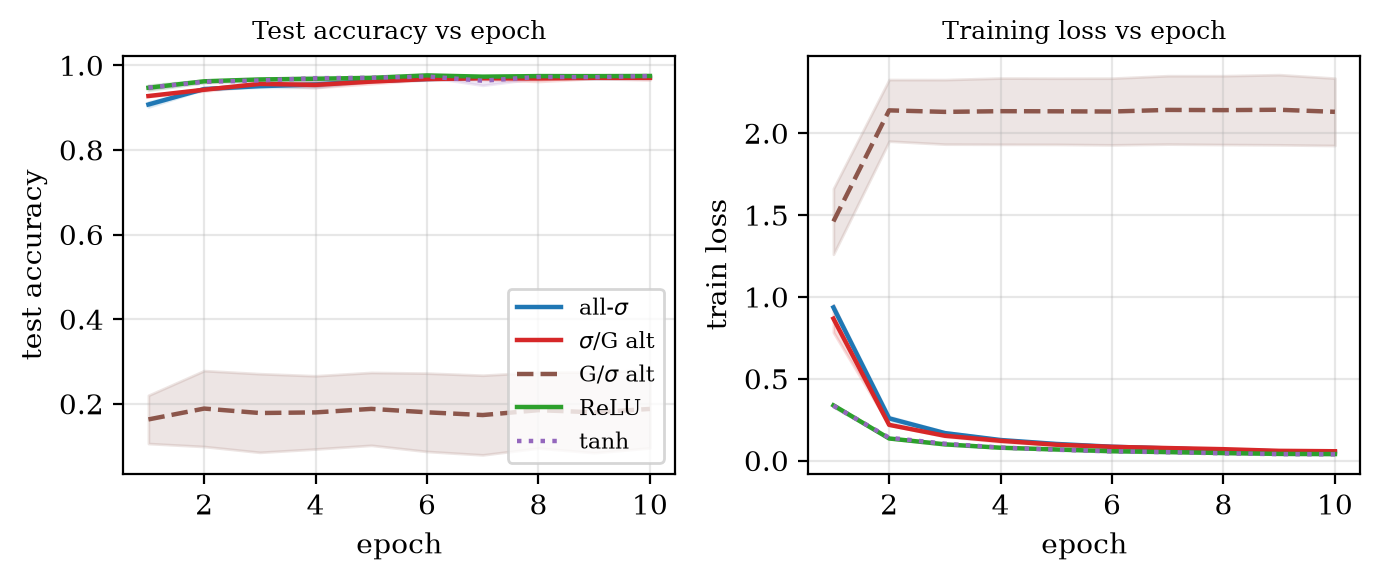
\includegraphics[width=0.95\textwidth]{../figures/fig3_training.png}
\caption{Training curves.  All four workable schemes (all-$\sigma$, $\sigma/G$,
ReLU, tanh) reach high accuracy, while $G/\sigma$ stalls at chance.}
\label{fig:train}
\end{figure}

\begin{figure}[t]
\centering
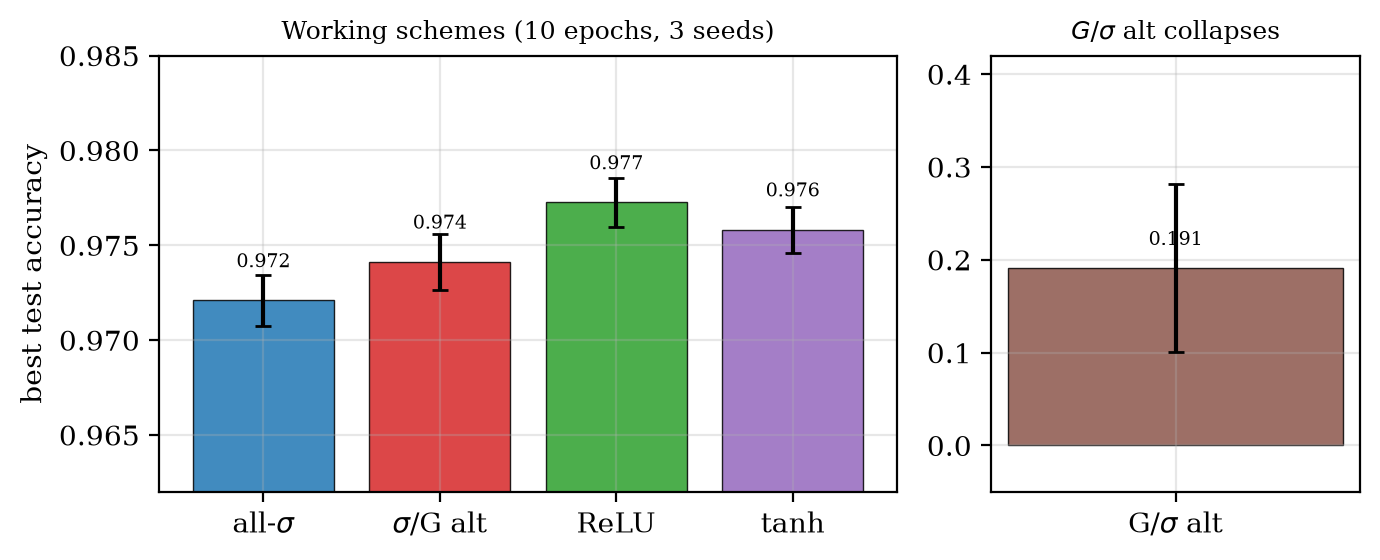
\includegraphics[width=0.95\textwidth]{../figures/fig4_accuracy_bar.png}
\caption{Best test accuracy (left, zoomed; right, the failed $G/\sigma$ scheme).
$\sigma/G$ alternation ($0.974$) outperforms all-$\sigma$ ($0.972$) and is
closest of the saturating schemes to ReLU/tanh.}
\label{fig:accbar}
\end{figure}

The gradient diagnostic in Table~\ref{tab:main} is the central evidence for the
hypothesis.  On a fresh, untrained network the gradient ratio for all-$\sigma$
is $3.37$---the input-side gradient is already an order of magnitude smaller
than the output-side gradient, i.e.\ gradients vanish as they propagate toward
the input.  For $\sigma/G$ alternation the same ratio is $1.03$ at
initialisation: the input- and output-side gradients are balanced to within a
few percent.  This is the direct empirical signature of the identity
$\sigma'(z)G'(z)\approx1$.  After training, all-$\sigma$ converges to $\sim1.1$
while $\sigma/G$ stays $\sim0.8$, so the balanced regime is maintained
throughout optimisation (Figure~\ref{fig:prodev}).

\begin{figure}[t]
\centering
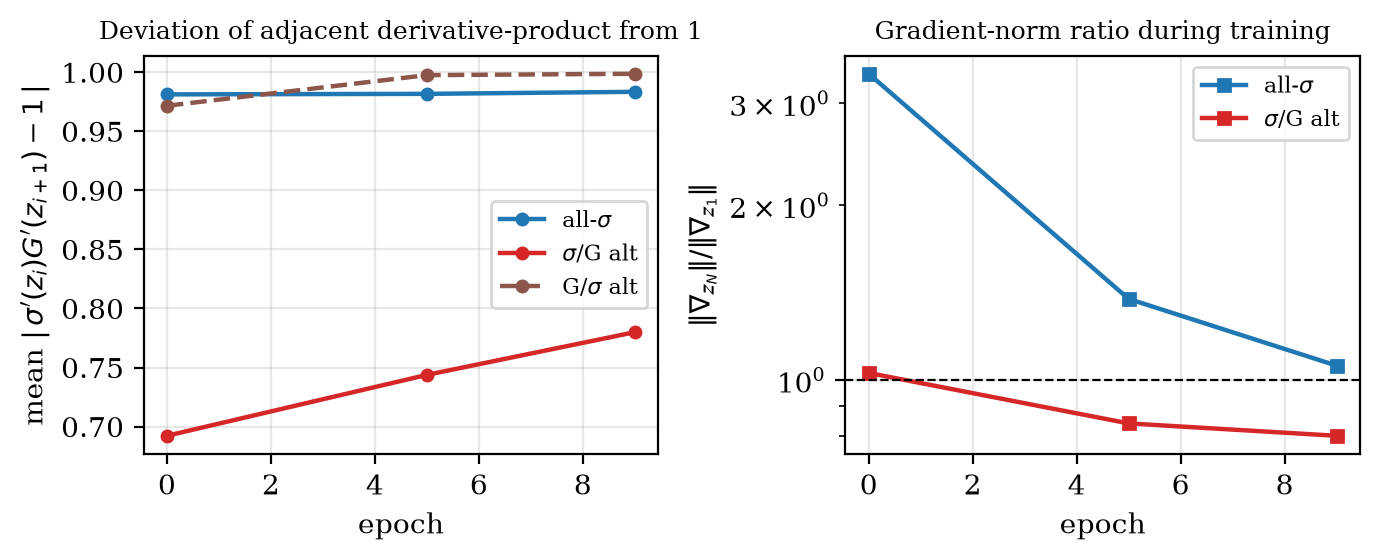
\includegraphics[width=0.95\textwidth]{../figures/fig6_prod_evolution.png}
\caption{Left: deviation of the adjacent derivative-product from $1$.  all-$\sigma$
\emph{multiplies} two factors $\sigma'(z_i)\sigma'(z_{i+1})\lesssim1/16$, so its
product is $\sim0.02$ (deviation $\sim0.98$).  $\sigma/G$ \emph{takes a ratio}
$\sigma'(z_i)/\sigma'(z_{i+1})$, which is bounded and $\mathcal{O}(1)$, so the
deviation is only $\sim0.7$.  Right: gradient-norm ratio over training---all-$\sigma$
starts imbalanced and $\sigma/G$ stays balanced.}
\label{fig:prodev}
\end{figure}

\subsection{Behaviour with depth}
\label{sec:results-depth}
The depth sweep isolates the vanishing/exploding mechanism
(Table~\ref{tab:depth}, Figure~\ref{fig:depth}).  all-$\sigma$ trains well only
for $L\lesssim6$; beyond $L=10$ the gradient ratio explodes by 2--16 orders of
magnitude and test accuracy collapses to chance.  $\sigma/G$ alternation extends
the trainable depth to $L\approx10$--$16$: the gradient ratio remains in
$[0.4,0.9]$ (close to $1$) throughout, and accuracy stays $\gtrsim0.96$ up to
$L=10$ and $\sim0.68$ at $L=16$, whereas all-$\sigma$ has already fallen to
$0.21$ at $L=10$ and $0.10$ at $L=16$.  ReLU is the most depth-robust (workable
to $L\approx24$), and tanh degrades at $L=32$.

\begin{table}[t]
\centering
\small
\caption{Depth sweep ($W=128$, 6 epochs).  acc = test accuracy, ratio =
$\|\partial L/\partial z_{L+1}\|/\|\partial L/\partial z_1\|$, $a_{\max}$ =
max activation magnitude.}
\label{tab:depth}
\begin{tabular}{lccccccc}
\toprule
scheme & $L$     & 2      & 4      & 6      & 10     & 16     & 32\\
\midrule
all-$\sigma$  & acc   & 0.963 & 0.955 & 0.920 & 0.211 & 0.103 & 0.114\\
              & ratio & 2.2  & 1.5  & 1.0  & $3.7\times10^{1}$ & $1.2\times10^{11}$ & $\infty$\\
              & $a_{\max}$ & 1.0 & 1.0 & 1.0 & 1.0 & 1.0 & 1.0\\
\midrule
$\sigma/G$    & acc   & 0.969 & 0.968 & 0.965 & 0.968 & 0.682 & 0.098\\
              & ratio & 0.72  & 0.80  & 0.83  & 0.89  & 0.40  & $1.1\times10^{8}$\\
              & $a_{\max}$ & 19 & 54 & 64 & 89 & $1.3\times10^{3}$ & 33\\
\midrule
ReLU          & acc   & 0.972 & 0.971 & 0.968 & 0.962 & 0.968 & 0.790\\
              & ratio & 0.66  & 0.60  & 0.52  & 0.50  & 0.51  & 0.73\\
              & $a_{\max}$ & 16 & 13 & 11 & 12 & 14 & $2.5\times10^{2}$\\
\midrule
tanh          & acc   & 0.972 & 0.969 & 0.970 & 0.970 & 0.952 & 0.114\\
              & ratio & 0.67  & 0.53  & 0.55  & 0.57  & 0.64  & $1.2\times10^{7}$\\
              & $a_{\max}$ & 1.0 & 1.0 & 1.0 & 1.0 & 1.0 & 1.0\\
\bottomrule
\end{tabular}
\end{table}

\begin{figure}[t]
\centering
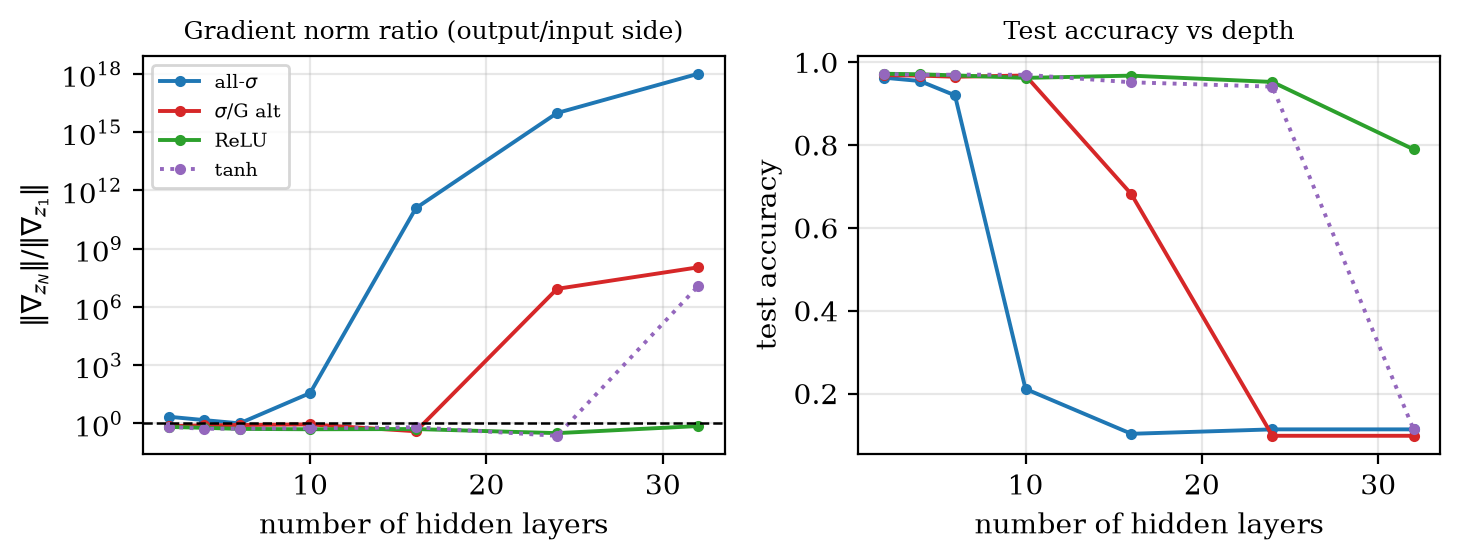
\includegraphics[width=0.95\textwidth]{../figures/fig5_depth_grad.png}
\caption{Gradient-norm ratio (left, log) and test accuracy (right) versus depth.
all-$\sigma$'s ratio explodes to $\sim10^{18}$ by depth $32$ while $\sigma/G$
stays $\mathcal{O}(1)$ to depth $16$; correspondingly all-$\sigma$ collapses at
$L\gtrsim10$ whereas $\sigma/G$ remains trainable to $L=16$.}
\label{fig:depth}
\end{figure}

\paragraph{The role of the unbounded activation $G$.}
The graded performance loss of $\sigma/G$ is not caused by vanishing gradients
but by \emph{forward activation growth}: $a_{\max}$ grows from $\sim19$ at $L=2$
to $\sim89$ at $L=10$ and $\sim1.3\times10^{3}$ at $L=16$
(Table~\ref{tab:depth}).  Once the pre-activations reach the exponential tail of
$G$, the following $\sigma$ layers saturate and the network becomes
untrainable---between $L=16$ and $L=24$ the gradient ratio suddenly jumps from
$0.40$ to $\sim10^{7}$.  Both all-$\sigma$ ($G$-free) and the exploded $G/\sigma$
ordering confirm the picture: the alternation $\sigma/G$ balances the derivative
product, but $G$'s unbounded forward map imposes a separate, depth-dependent
ceiling.  This is quantified in Figure~\ref{fig:perlayer} for $L=6$: at initialisation
all-$\sigma$ gradients span four orders of magnitude across layers ($10^{-5}$ to
$10^{-1}$) whereas $\sigma/G$ gradients vary by only about one order.

\begin{figure}[t]
\centering
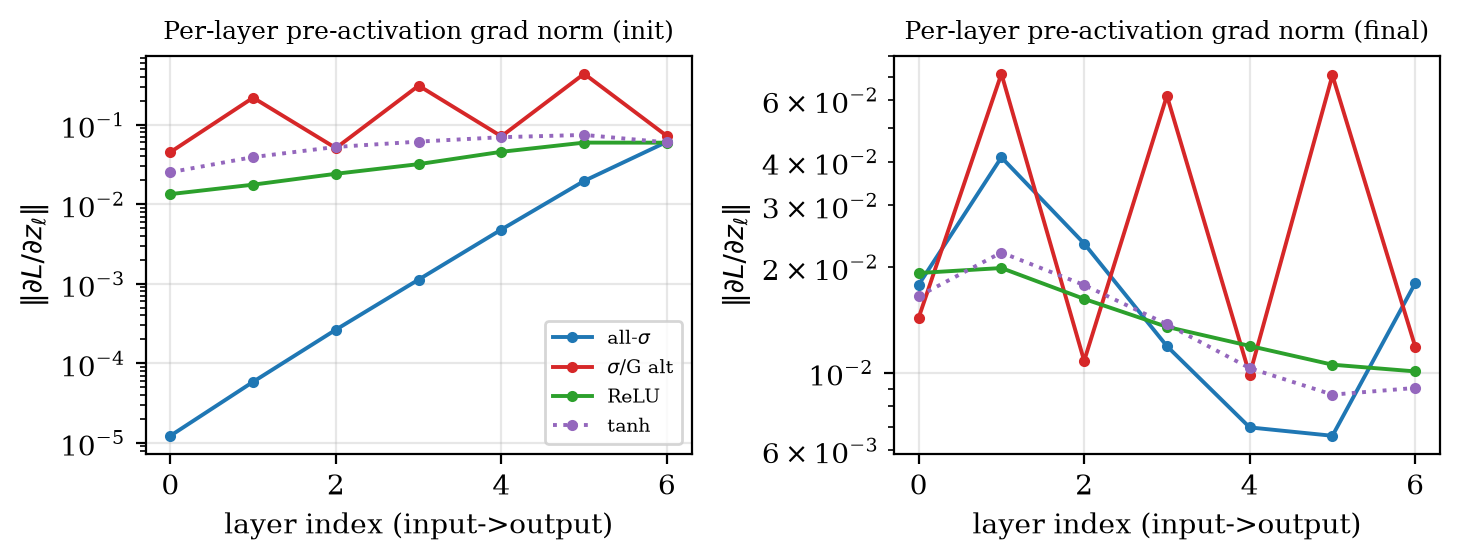
\includegraphics[width=0.95\textwidth]{../figures/fig7_per_layer_grad.png}
\caption{Per-layer pre-activation gradient norms at $L=6$.  At initialisation
(left) all-$\sigma$ spans $\sim4$ decades while $\sigma/G$ is flat; after training
(right) the $\sigma/G$ profile oscillates because $\sigma$ and $G$ layers carry
different derivative scales.}
\label{fig:perlayer}
\end{figure}

\subsection{What the figures show about the identity}
\label{sec:results-product}
Figure~\ref{fig:act} (left) shows $\sigma$ and $G$ together with their
derivatives; the product $\sigma'(z)G'(z)$ is exactly $1$ for every $z$
(Figure~\ref{fig:identity}, left), so an alternating pair is a perfect
derivative-rescaling of the sigmoid.  The right panel of
Figure~\ref{fig:identity} shows the trade-off: the product
$\sigma'(z_i)G'(z_{i+1})=\sigma'(z_i)/\sigma'(z_{i+1})$ deviates from $1$
\emph{only} through the mismatch $\Delta z=z_i-z_{i+1}$, growing exponentially
in $\Delta z$ with a rate $1-2\sigma(z_{i+1})$ that vanishes for saturated
pre-activations.

\begin{figure}[t]
\centering
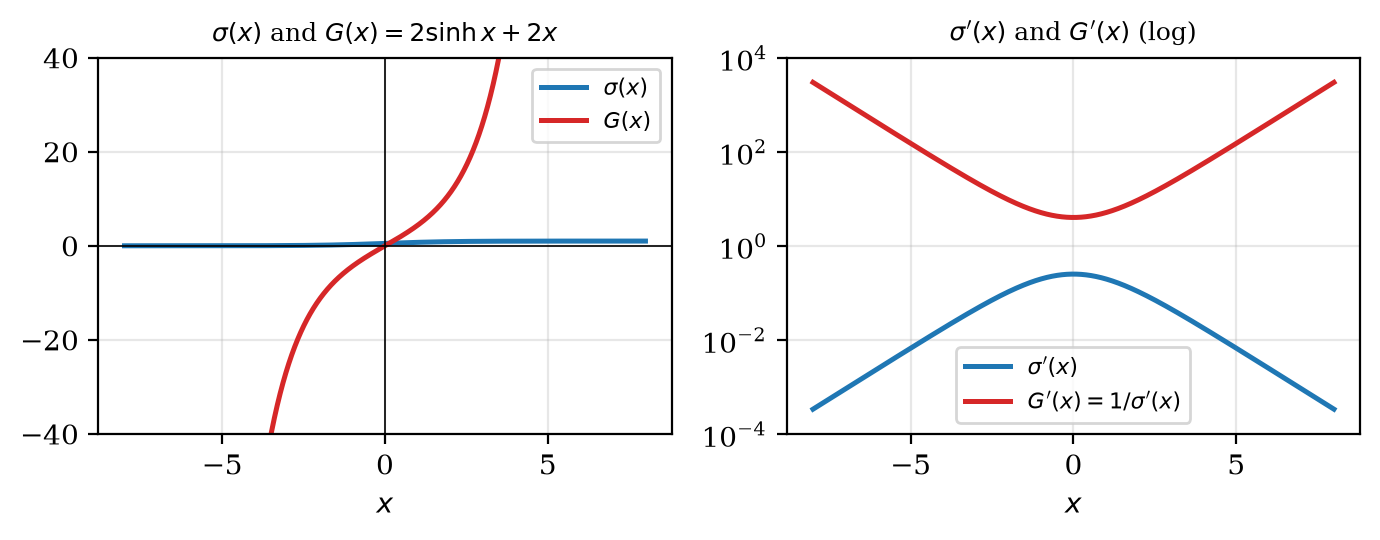
\includegraphics[width=0.95\textwidth]{../figures/fig1_activations.png}
\caption{Left: $\sigma$ (bounded) and the reciprocal-derivative antiderivative
$G(x)=2\sinh x+2x$ (unbounded, exponential).  Right: $\sigma'$ and
$G'=1/\sigma'$; note the exact symmetry about $x=0$.}
\label{fig:act}
\end{figure}

\begin{figure}[t]
\centering
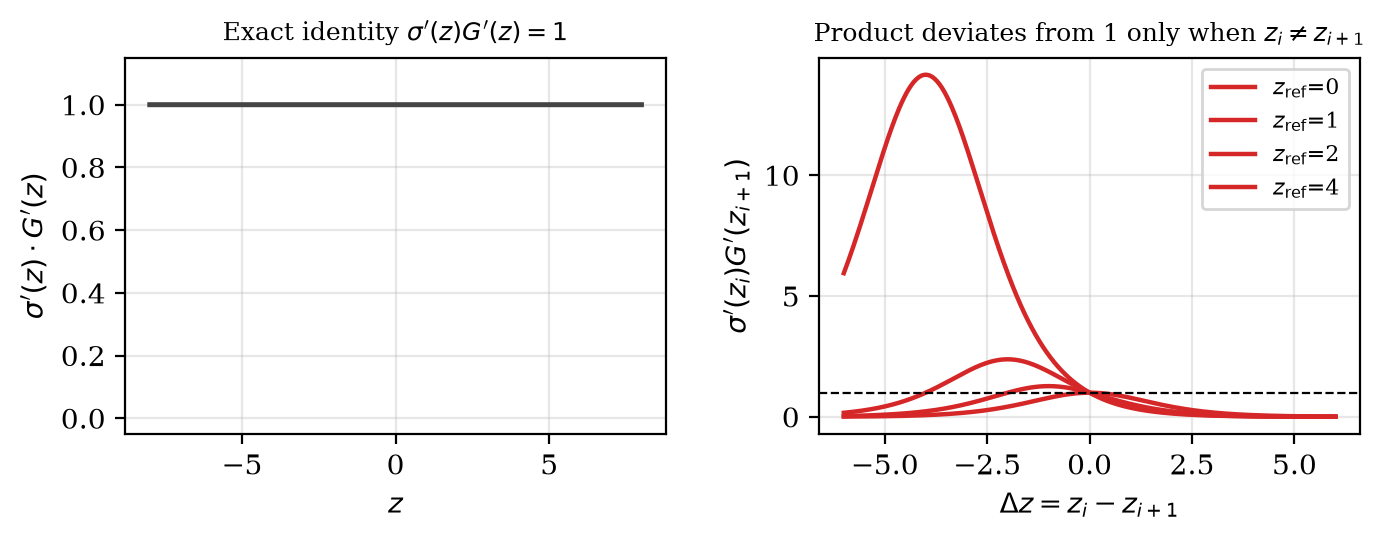
\includegraphics[width=0.95\textwidth]{../figures/fig2_derivative_identity.png}
\caption{Left: the exact identity $\sigma'(z)G'(z)=1$.  Right: the product
$\sigma'(z_i)G'(z_{i+1})$ equals $1$ when $z_i=z_{i+1}$ and departs from $1$
exponentially as the mismatch $\Delta z=z_i-z_{i+1}$ grows.}
\label{fig:identity}
\end{figure}

\section{Discussion}
\label{sec:discussion}
The results support the hypothesis in a precise, though bounded, sense.
Three facts stand out.  First, the identity is exact and algebraic:
$G'(x)=1/\sigma'(x)$, so an adjacent $(\sigma,G)$ pair contributes
$\sigma'(z_i)/\sigma'(z_{i+1})$ to the backprop chain---a ratio of two
bounded numbers rather than a product.  This turns a quantity that is
\emph{guaranteed} small ($\sigma'(z_i)\sigma'(z_{i+1})\le1/16$) into one that is
$\mathcal{O}(1)$.  Second, the measured gradient ratio at initialisation is
$1.03$ for $\sigma/G$ versus $3.37$ for all-$\sigma$, and $\sigma/G$ keeps the
ratio near $1$ both during training and to substantially greater depth
(Figure~\ref{fig:depth}).  Third, the ordering matters: $G$ must follow
$\sigma$.  Starting with $G$ ($G/\sigma$) sends the activations to
$\sim10^{11}$ and the network to chance, because an unbounded expansion at the
input is not preceded by a compression.

The enhancement is real but not a panacea.  Whereas all-$\sigma$ dies from
vanishing gradients, $\sigma/G$ dies from the exponential forward growth of the
$G$ activation itself.  The alternation cannot remove this: even with a perfect
derivative product, if the signal magnitude entering $G$ grows with depth, the
next $\sigma$ layer saturates and the network loses the ability to propagate
signal.  A natural remedy is to make the $\sigma/G$ alternation
scale-preserving, e.g.\ by restricting $G$ to a bounded window
($G(x)\approx2x$ for small $x$) or by normalising the activations; we do not
pursue this here.

\section{Limitations}
\label{sec:limits}
This is a small-scale study on MNIST with a fully-connected architecture and a
short training budget (6--10 epochs); conclusions may not transfer to
large-scale or convolutional networks.  The comparison uses identical
Xavier initialisation and Adam for every scheme, so the $\sigma/G$ network is
not tuned to the larger scale of $G$'s outputs.  Only five activation schemes
and a single network width were tested.  The depth sweep uses one seed.

\section{Conclusion}
\label{sec:conclusion}
We introduced and analysed the Sigmoid--G Alternating Activation (SGAA):
interleaving the logistic sigmoid $\sigma$ with the antiderivative of the
reciprocal derivative, $G(x)=2\sinh x+2x$, so that $G'(x)=1/\sigma'(x)$.  The
adjacent derivative product becomes a ratio $\sigma'(z_i)/\sigma'(z_{i+1})$,
which is exactly $1$ for equal pre-activations and remains $\mathcal{O}(1)$
otherwise.  On MNIST, $\sigma/G$ alternation outperforms all-$\sigma$ (test
accuracy $0.974$ vs.\ $0.972$), keeps the input- to output-side gradient ratio
at $\approx1$ from initialisation, and extends the trainable depth roughly
twofold, while the $G/\sigma$ ordering fails catastrophically.  The main
limitation is the unbounded forward growth of $G$, which bounds the achievable
depth.  Future work will consider scale-preserving variants of the $\sigma/G$
pair and application to deeper, convolutional architectures.

\bibliographystyle{plain}
\begin{thebibliography}{9}
\bibitem{goodfellow} Goodfellow, Bengio, Courville (2016). \emph{Deep Learning}. MIT Press.
\bibitem{glorot2010} Glorot, Bengio (2010). Understanding the difficulty of training deep feedforward neural networks. \emph{AISTATS}.
\bibitem{he2015} He, Zhang, Ren, Sun (2015). Delving deep into rectifiers. \emph{ICCV}.
\bibitem{kingma2015} Kingma, Ba (2015). Adam: A method for stochastic optimization. \emph{ICLR}.
\end{thebibliography}

\end{document}
